% Why the reported quantile has to be smoothed.
%   left  -- the plain estimator picks one order statistic; its gradient rests
%            on a single patient and jumps when two swap rank.
%   right -- Beta(kappa, n-kappa+1) weights in cumulative-weight space: exactly
%            the expectation the model has to predict, and differentiable.
% Heights on the right are f_B(c_i; 3, 7) at c_i = (i-1/2)/9, scaled to 1.
%
%   compile:  pdflatex smooth_quantile.tex
%
\documentclass[border=10pt]{standalone}
\usepackage{lmodern}
\usepackage{amsmath}
\usepackage{amssymb}
\usepackage{tikz}
\usetikzlibrary{arrows.meta,positioning}
% Shared palette for the population-model figures.
%   ink      body / structure
%   popcol   the patient cloud and anything predicted from it
%   mechcol  the simulator and species-level quantities
%   msrcol   the measurement map (readout-level: gamma, kappa)
%   datacol  reported rows
\definecolor{ink}{HTML}{3A3A3A}
\definecolor{popcol}{HTML}{3B4AA6}
\definecolor{mechcol}{HTML}{2E7D5B}
\definecolor{msrcol}{HTML}{EB811B}
\definecolor{datacol}{HTML}{8C3B4A}


\begin{document}
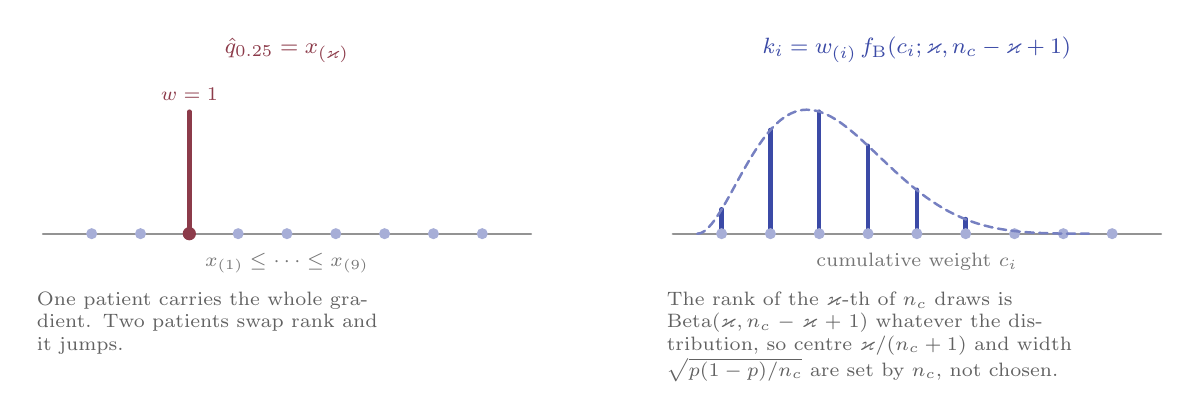
\begin{tikzpicture}[
  font=\sffamily, >=Stealth, line cap=round, line join=round,
  ttl/.style={font=\footnotesize\bfseries, anchor=south},
  figcap/.style={font=\scriptsize, text=ink!80, align=left, anchor=north west}]

\def\S{0.62}   % patient spacing

% ================================================================ left panel
\begin{scope}[shift={(0,0)}]
  \draw[ink!55, line width=0.8pt] (0.3,0) -- ({0.3+10*\S},0);
  \foreach \i in {1,...,9} \fill[popcol!45] ({0.3+\i*\S},0) circle (2pt);
  % the selected order statistic
  \draw[datacol, line width=1.6pt] ({0.3+3*\S},0) -- ({0.3+3*\S},1.55);
  \fill[datacol] ({0.3+3*\S},0) circle (2.4pt);
  \node[datacol, font=\scriptsize, anchor=south] at ({0.3+3*\S},1.57) {$w=1$};
  \node[ink!70, font=\scriptsize, anchor=north] at ({0.3+5*\S},-0.12)
    {$x_{(1)}\le\cdots\le x_{(9)}$};
  \node[ttl, datacol] at ({0.3+5*\S},2.05) {$\hat q_{0.25}=x_{(\varkappa)}$};
\end{scope}
\node[figcap, text width=44mm] at (0.1,-0.62)
  {One patient carries the whole gradient. Two patients swap rank and it jumps.};

% ================================================================ right panel
\begin{scope}[shift={(8.0,0)}]
  \draw[ink!55, line width=0.8pt] (0.3,0) -- ({0.3+10*\S},0);
  \foreach \i/\h in {1/0.20, 2/0.85, 3/1.00, 4/0.72, 5/0.36, 6/0.12, 7/0.02, 8/0.00, 9/0.00}{
    \draw[popcol, line width=1.6pt] ({0.3+\i*\S},0) -- ({0.3+\i*\S},{1.55*\h});
    \fill[popcol!45] ({0.3+\i*\S},0) circle (2pt);}
  % the Beta density the weights come from
  \draw[popcol!70, densely dashed, line width=0.9pt]
    plot[domain=0.5:8.6,samples=110,smooth]
      ({0.3+\x*\S},{1.55*252*((\x-0.5)/9)^2*(1-(\x-0.5)/9)^6/2.759});
  \node[ttl, popcol] at ({0.3+5*\S},2.05)
    {$k_i=w_{(i)}\,f_{\mathrm{B}}\!\left(c_i;\varkappa,n_c-\varkappa+1\right)$};
  \node[ink!70, font=\scriptsize, anchor=north] at ({0.3+5*\S},-0.12)
    {cumulative weight $c_i$};
\end{scope}
\node[figcap, text width=52mm] at (8.1,-0.62)
  {The rank of the $\varkappa$-th of $n_c$ draws is $\mathrm{Beta}(\varkappa,n_c-\varkappa+1)$
   whatever the distribution, so centre $\varkappa/(n_c+1)$ and width
   $\sqrt{p(1-p)/n_c}$ are set by $n_c$, not chosen.};

\end{tikzpicture}
\end{document}
